\begin{figure}[t]
\centering
%\begin{tabular}{cc}
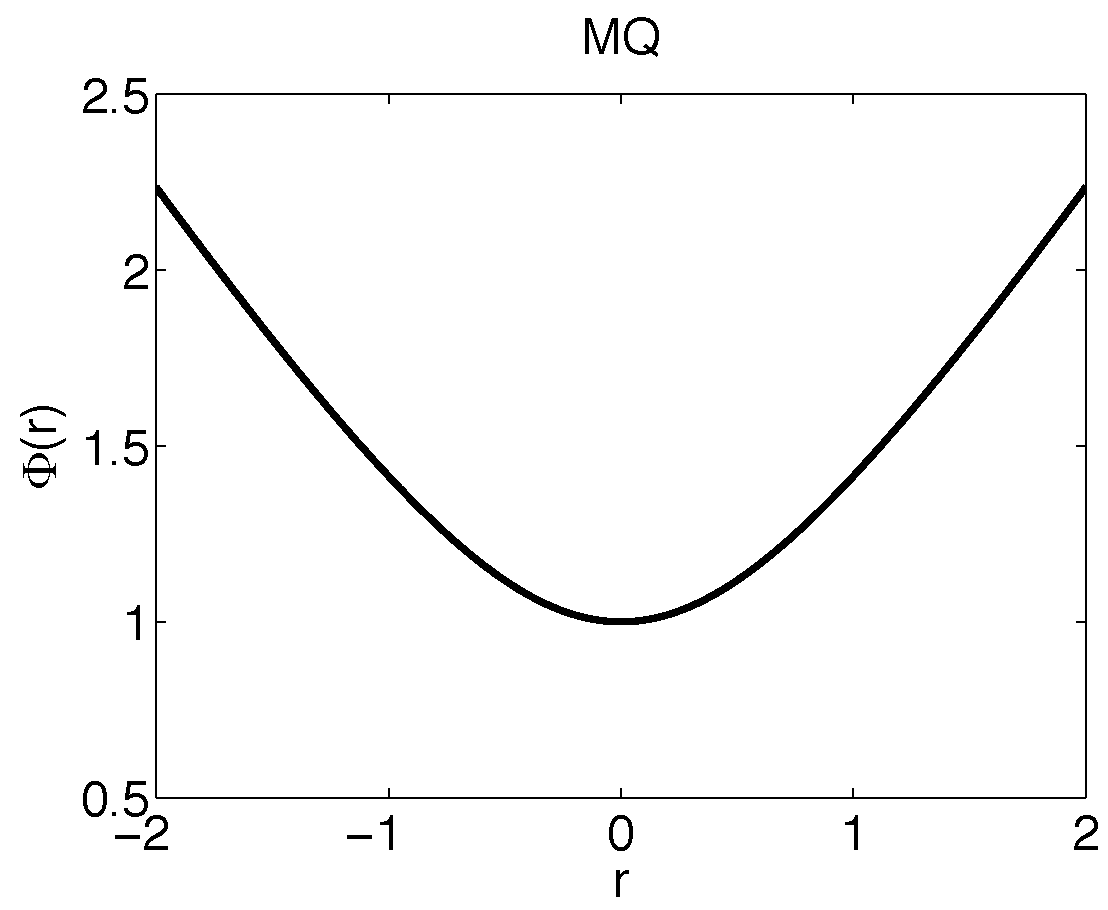
\includegraphics[width=0.25\textwidth]{matlab/mq_rbf.pdf}   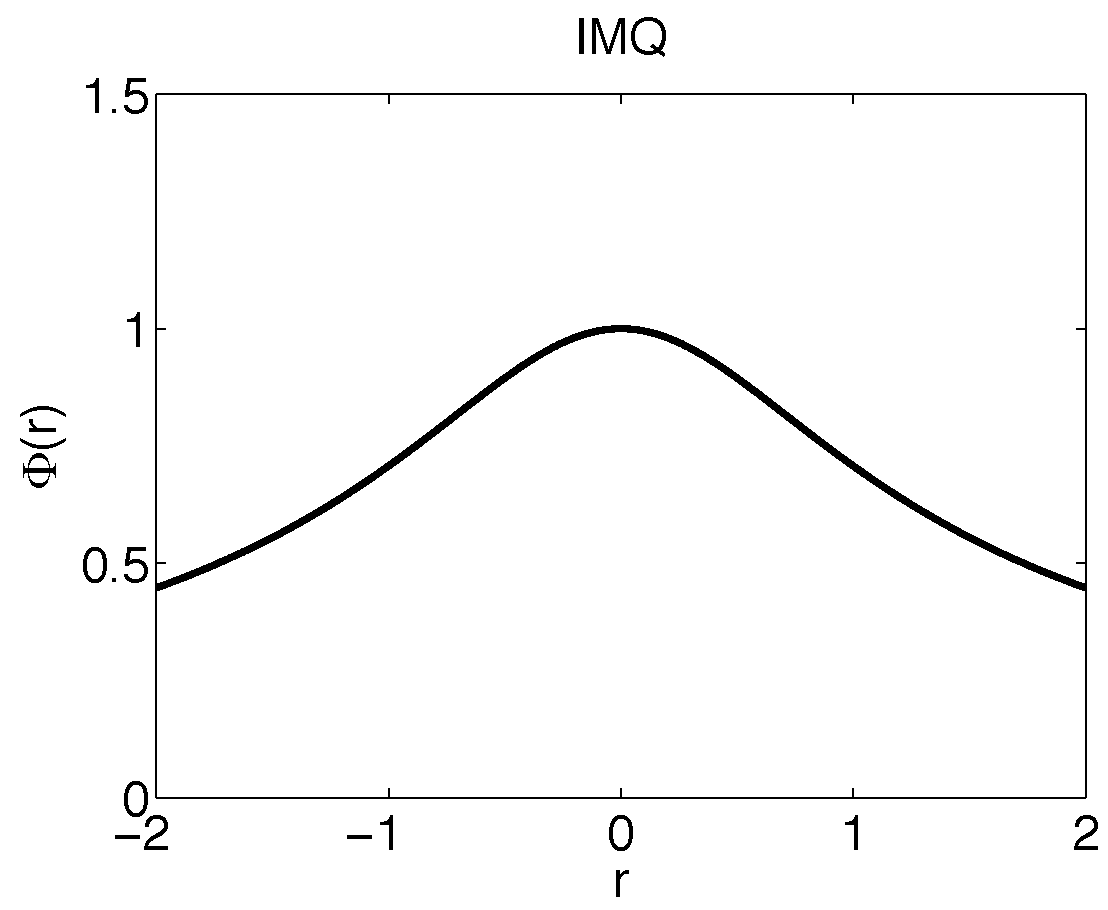
\includegraphics[width=0.25\textwidth]{matlab/imq_rbf.pdf} 
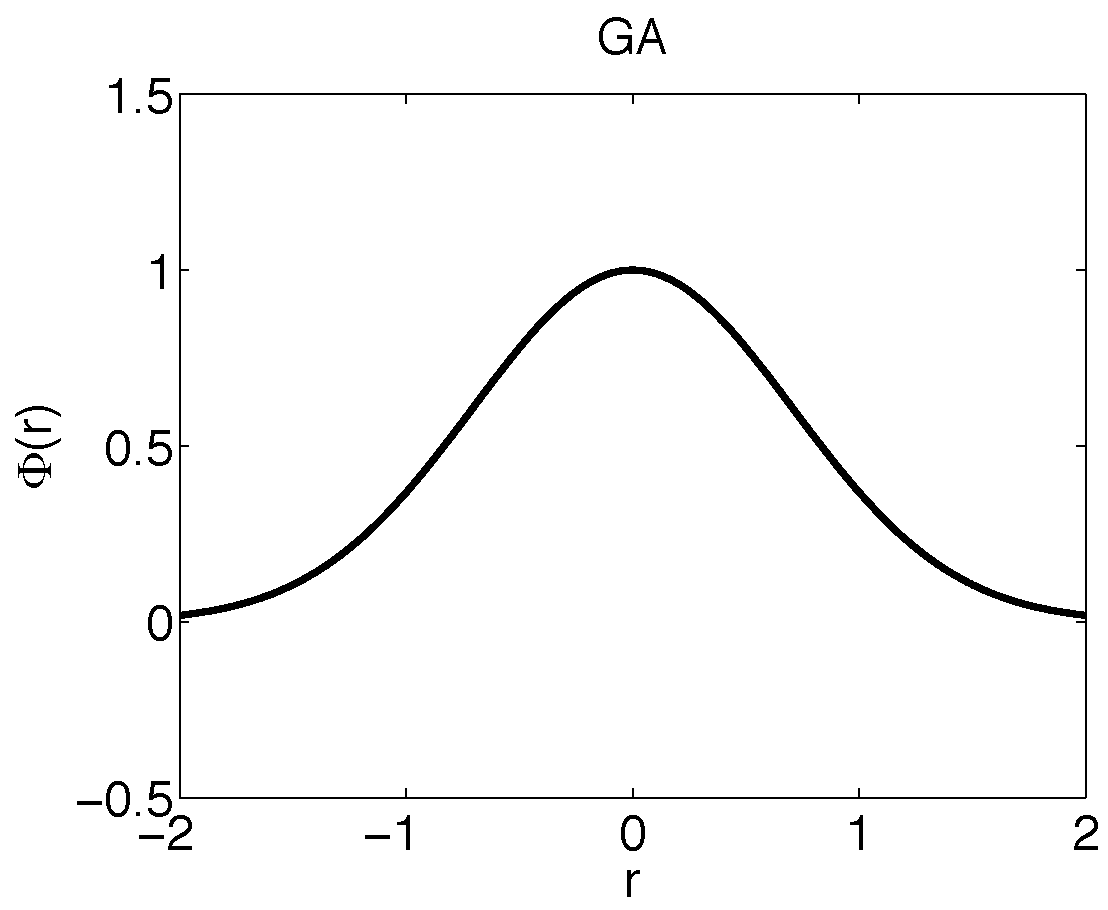
\includegraphics[width=0.25\textwidth]{matlab/ga_rbf.pdf} \\  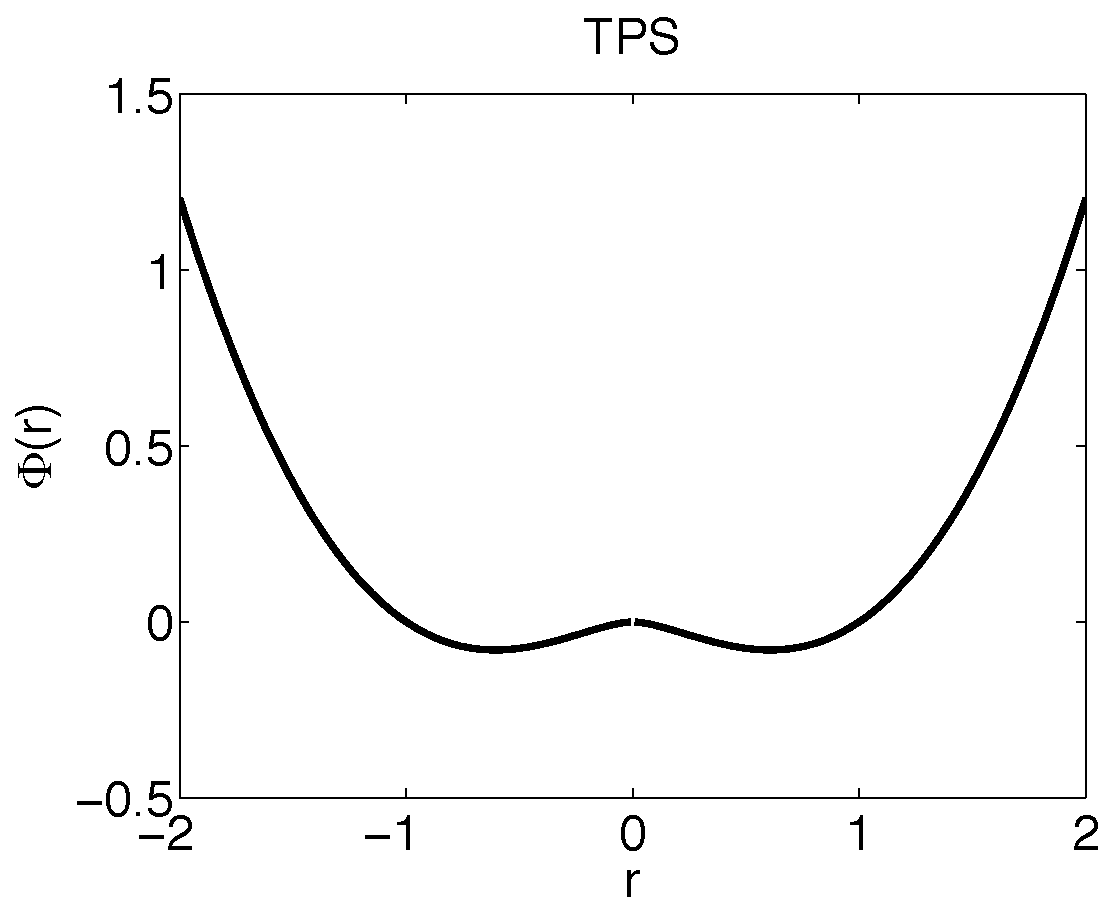
\includegraphics[width=0.25\textwidth]{matlab/tps_rbf.pdf} 
%\end{tabular} \\
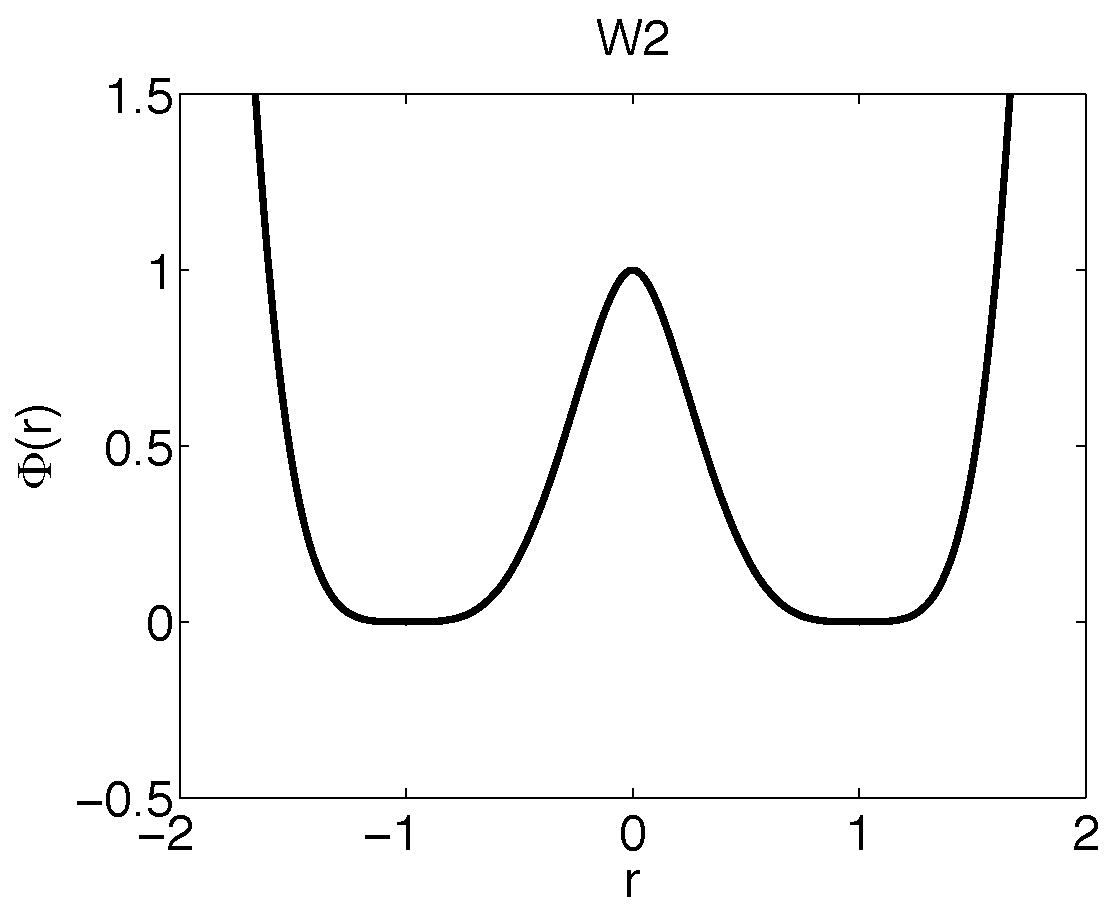
\includegraphics[width=0.25\textwidth]{matlab/w2_rbf.pdf}
\caption{Example RBF shapes from Table~\ref{tbl:rbfs} with parameter $\varepsilon=1$.}
\label{fig:rbf_examples}
\end{figure} 


\begin{figure}[t]
\centering
\begin{tabular}{cc}
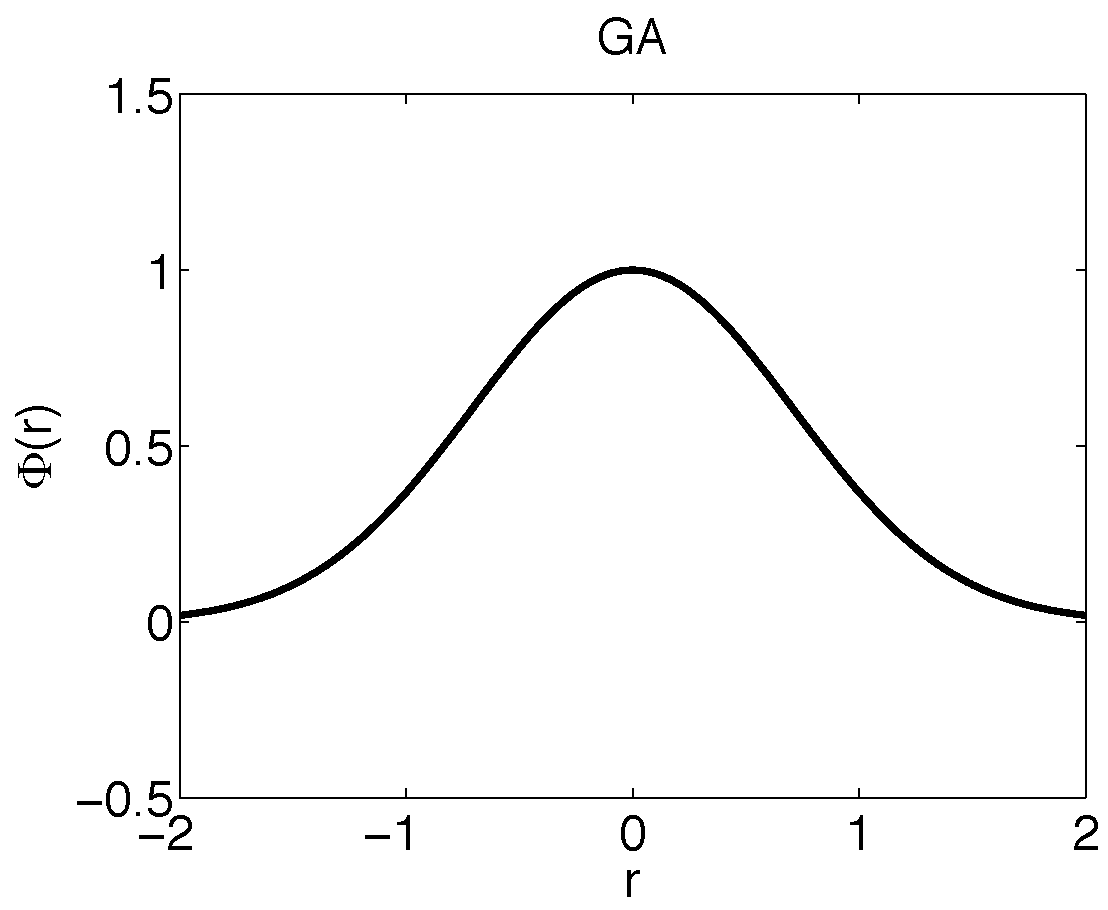
\includegraphics[width=0.275\textwidth]{matlab/ga_rbf.pdf}
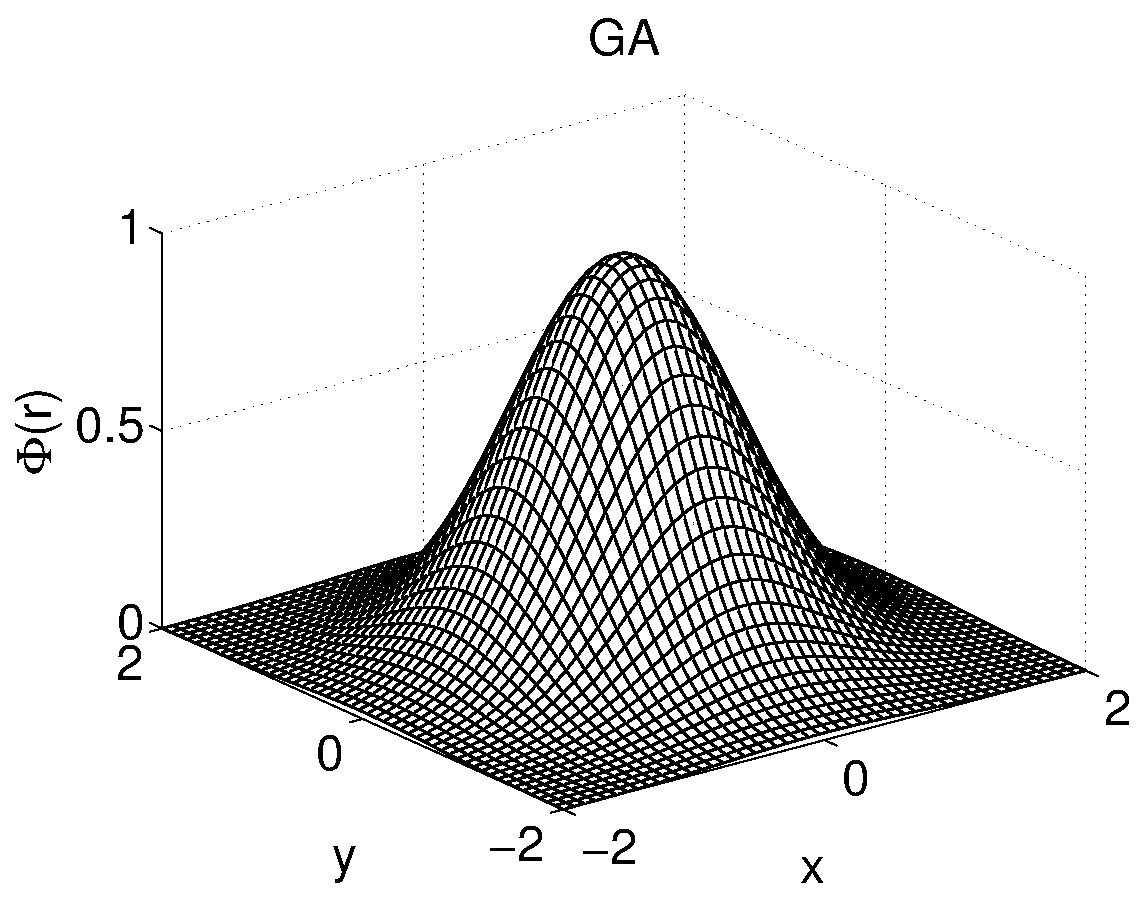
\includegraphics[width=0.3\textwidth]{matlab/ga_rbf2D-eps-converted-to.pdf}
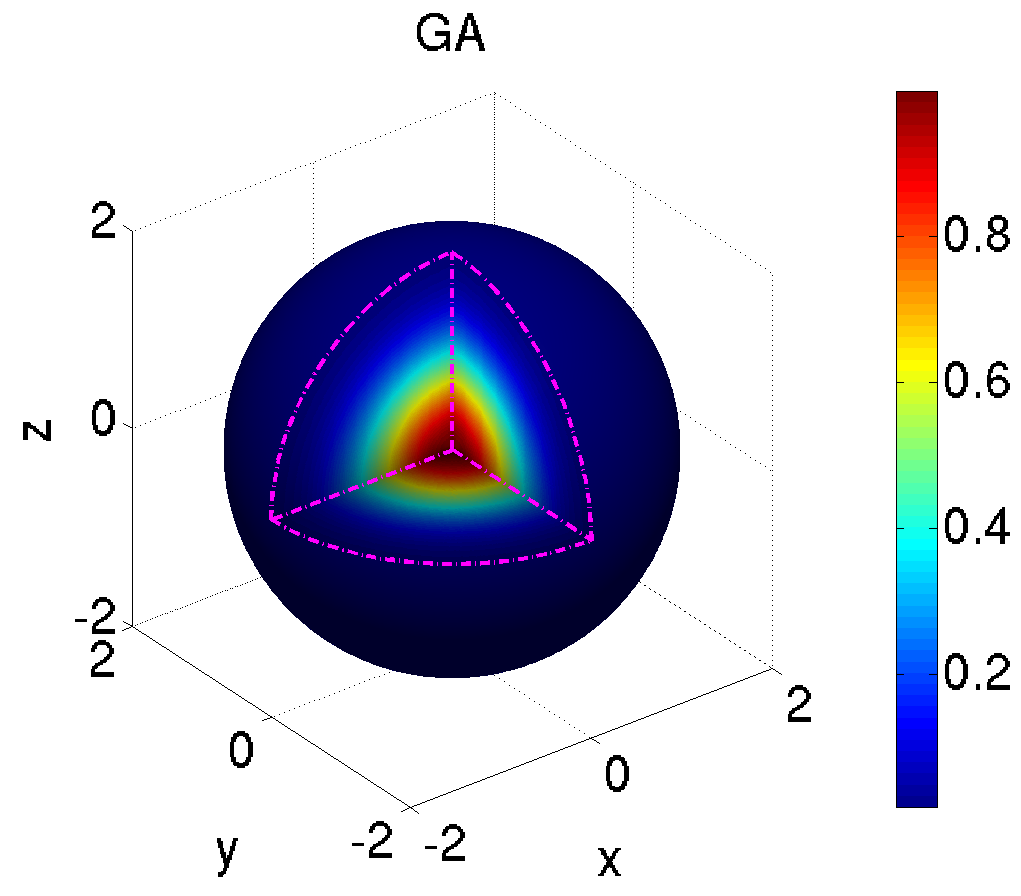
\includegraphics[width=0.3\textwidth]{matlab/ga_rbf3D-eps-converted-to.pdf}
\end{tabular} 
\caption{The Gaussian (GA) RBF (Table~\ref{tbl:rbfs}) with parameter $\varepsilon=1$ and $r$ in $D = 1$, $2$ and $3$.}
\label{fig:rbf_dimension_example}
\end{figure} 
